\documentclass[conference]{IEEEtran}
\IEEEoverridecommandlockouts
% The preceding line is only needed to identify funding in the first footnote. If that is unneeded, please comment it out.
\usepackage{cite}
\usepackage{amsmath,amssymb,amsfonts}
\usepackage{algorithmic}
\usepackage{graphicx}
\usepackage{textcomp}
\usepackage{xcolor}
\def\BibTeX{{\rm B\kern-.05em{\sc i\kern-.025em b}\kern-.08em
    T\kern-.1667em\lower.7ex\hbox{E}\kern-.125emX}}
\begin{document}

\title{Final Project: Improve SHIP++ cache replacement policy}

\author{
Miaoxiang Yu, Yiming Du\\
University of Rhode Island\\
\{miaoxiang\_yu, yiming\}@uri.edu
}

\maketitle

\begin{abstract}
In modern computer architecture, cache plays a critical role in bridging the performance gap between high-speed processors and main memory. With the increasing use of chip multiprocessors and shared last-level caches (LLCs), effective cache replacement policies are essential for maintaining high-performing LLCs. This paper focuses on enhancing cache performance by examining the SHIP++ cache replacement policy, which combines the Signature History Counter Table (SHCT) and bypass techniques. SHIP++ addresses the challenges posed by cache trashing and ineffective bypassing when the majority of reuse distances surpass the number of cache ways in a set. By quantifying the number of valuable data elements and employing bypassing techniques based on SHCT analysis, SHIP++ makes efficient use of cache space and improves cache hit rates. The proposed approach is evaluated on a range of benchmarks, demonstrating improved cache performance compared to the original SHIP. Furthermore, the paper explores strategies for optimizing the utilization of the SHCT table, including adaptive sizing, intelligent initialization, and hybrid approaches, leading to more accurate cache replacement decisions and enhanced overall system performance.
\end{abstract}

\begin{IEEEkeywords}
ship, ship++, bypass, cache replacement policy
\end{IEEEkeywords}

% Introduction

\section{Introduction}
In the ever-evolving world of computer architecture, cache serves as an essential intermediary storage tier within the memory hierarchy of contemporary computer architectures. Its primary function is to bridge the significant speed disparity between high-performance processors and main memory. The prevalent utilization of chip multiprocessors with shared last-level caches (LLCs) and the growing divergence between the processor and memory speeds further underscores the necessity for high-performing LLCs in modern computing systems\cite{Wu2011}. Recent research findings indicate that the widely-adopted Least Recently Used (LRU) replacement policy possesses considerable potential for performance enhancement. Consequently, a substantial corpus of scholarly investigations has concentrated on refining last-level cache (LLC) replacement techniques to further optimize system performance\cite{Gao2010,Seznec2010}. This manuscript emphasizes the enhancement of cache performance through the integration of the Signature History Counter Table (SHCT) and bypass methodologies, thereby striving to achieve a more efficient cache management system.\par
The Least Recently Used (LRU) cache replacement policy is a widely adopted and well-established technique in computer architecture. The origins of LRU can be traced back to the early days of cache memory implementation in the 1960s and 1970s. Over the years, it has become a fundamental cache management policy due to its simplicity and effectiveness. The LRU algorithm operates on the premise that the least recently accessed data is less likely to be required in the near future. In other words, when a cache replacement becomes necessary, the LRU policy selects the cache block that has not been accessed for the longest time to be evicted. To achieve this, LRU maintains a record of the access history of the cache blocks, typically by updating a timestamp or rearranging a list of blocks according to their usage. The LRU cache replacement policy is straightforward to understand and implement. Simultaneously, it can adapt to varying access patterns, as it inherently takes into account the recent history of cache block usage. In many cases, LRU delivers satisfactory cache hit rates, resulting in efficient system performance. However, its disadvantage is obvious, it solely relies on past access patterns and does not consider any potential future access patterns, which can sometimes result in suboptimal cache block replacement decisions. Concurrently, maintaining access history for cache blocks may require additional data structures and processing, increasing the overhead of cache management. Furthermore, in scenarios with unique access patterns, such as cyclic or large working sets, the LRU policy may not perform as efficiently as other specialized replacement policies\cite{Gao2010,Seznec2010,Khan2010,Daniel2010,Kharbutli2008,Qureshi2007,santh2007,C2010,Sigarch2009}.\par
The Signature-based Hit Predictor (SHIP) cache replacement policy is an advanced technique introduced by A. Jaleel et al\cite{Seznec2010}. SHIP aims to address some of the limitations of traditional cache replacement policies, such as the Least Recently Used (LRU) algorithm, by employing a more sophisticated approach to cache management. SHIP operates by predicting the re-reference interval of a cache block, which is the number of accesses between two consecutive accesses of the same block. The re-reference interval is used to determine the eviction priority of cache blocks. SHIP utilizes a data structure called the Signature History Counter Table (SHCT) to store the history of re-reference intervals for each cache block, indexed by a signature derived from the block's address. When a cache block is accessed, SHIP computes its signature and updates the corresponding SHCT entry. The re-reference interval prediction is then employed to assign a Recency Position (RP) value to the cache block. Cache blocks with higher RP values are considered less likely to be accessed in the near future and are prioritized for eviction. It can improve the cache hit rate by predicting the re-reference interval. SHIP can better anticipate future access patterns, leading to higher cache hit rates compared to traditional policies like LRU. Coincident, SHIP can adapt to various access patterns by dynamically updating the re-reference interval predictions based on observed behavior. The SHIP algorithm is designed to work effectively with different cache sizes and associativities, making it a versatile solution for diverse system configurations. However, the SHIP cache replacement policy also has certain disadvantages, like the prediction mechanism and SHCT management in SHIP add complexity to the cache management process compared to simpler policies like LRU. Maintaining the SHCT and implementing the re-reference interval prediction mechanism require additional memory and processing resources, which could potentially offset the performance benefits. While SHIP aims to predict future access patterns, it is not infallible, and prediction errors may lead to suboptimal cache block replacement decisions.\cite{Wu2011}\par





% Principles

\section{Background}
\subsection{Background of SHiP}
Signature-based hit predictor(SHiP) is a method used in high-performance caching systems to predict cache hits based on signatures of memory access patterns. In this approach, the cache is divided into multiple signature-based prediction modules, each responsible for a subset of memory accesses. The signature module creates a signature for each memory access and stores it in the cache. The hit predictor then uses these signatures to predict future cache hits, based on a match between the current memory access signature and the stored signatures. This method allows for faster cache hit detection and reduced access latencies, as the hit predictor can quickly retrieve data from the cache without accessing the main memory\cite{llc}. Signature-based hit predictor is particularly useful in large-scale computing systems that require high-performance caching to handle large amounts of data and reduce access latencies. It is also a popular method for multi-core and multi-processor systems, as it allows for efficient and scalable cache management across multiple computing nodes\cite{Jinchun,Elvira}.

 The history of signature-based hit predictor dates back to the early 1990s, when researchers began exploring ways to improve the performance of computer memory systems. The first signature-based hit predictor was introduced in a paper published by IBM researchers in 1993. This system used a signature-based approach to predict cache hits, in which a small signature was generated for each memory access and used to predict future access patterns. This system was able to achieve significant improvements in cache performance and reduced access latencies, making it a popular technology in high-performance computing systems.\cite{Samira} Over the next few years, researchers continued to refine the signature-based hit predictor technology, developing new algorithms and techniques for improving prediction accuracy and reducing latency. One of the key advances during this time was the introduction of the two-level signature-based hit predictor, which incorporated two levels of signature generation and prediction to improve the accuracy of cache hit predictions. In the early 2000s, researchers began exploring the use of machine learning techniques in signature-based hit predictor systems. These techniques used statistical models and pattern recognition algorithms to learn and predict access patterns based on historical data, improving the accuracy of cache hit predictions even further. In recent years, researchers have continued to refine and improve signature-based hit predictor systems, incorporating new features and parameters to optimize performance in modern multi-core and multi-processor systems. These include processor affinity tracking, access history and frequency tracking, and other parameters specific to parallel computing architectures. Today, signature-based hit predictor is widely used in high-performance computing systems, including supercomputers, data centers, and cloud computing environments.\cite{Wu2011} It is an important technology for improving the performance and efficiency of modern computing systems and is likely to remain an area of active research and development in the coming years.

\subsection{Background of SHiP++}
Signature-based hit predictor++ is an advanced method for predicting cache hits that builds upon the traditional signature-based hit predictor method used in high-performance caching systems.\cite{San,arka} This method is designed to improve cache efficiency and performance in multi-core and multi-processor systems by predicting cache hits based on multiple parameters and features.\cite{Samira} The basic idea behind signature-based hit predictor++ is to divide the cache into multiple prediction modules, each responsible for a subset of memory accesses.\cite{ADueling} Each module generates a signature for each memory access and stores it in the cache. The hit predictor++ then uses these signatures to predict future cache hits, based on a match between the current memory access signature and the stored signatures. However, unlike traditional signature-based hit predictor, which uses only the memory access pattern to predict cache hits, signature-based hit predictor++ incorporates additional features and parameters to improve the accuracy of predictions\cite{Belady}.\par

One of the key features of SHiP++ is its ability to predict cache hits based on processor affinity \cite{Evan}. In multi-core and multi-processor systems, different processors or cores may have different access patterns and may be more likely to access certain areas of memory than others. Signature-based hit predictor++ takes this into account by tracking the processor affinity of each memory access and using this information to predict cache hits. This improves the accuracy of predictions and helps to reduce access latencies. Another important feature of signature-based hit predictor++ is its ability to predict cache hits based on access history and frequency. By tracking the history of memory accesses and the frequency of access to different areas of memory, signature-based hit predictor++ can make more accurate predictions about which data is likely to be accessed in the future. This feature is particularly useful in multi-core and multi-processor systems, where multiple processors may be accessing the same areas of memory at different times. In addition to these features, signature-based hit predictor++ also incorporates other parameters and features that are specific to multi-core and multi-processor systems, such as cache partitioning, interconnect bandwidth, and cache coherence protocols. These parameters are used to optimize cache performance and reduce access latencies, particularly in systems with high levels of parallelism and complex memory access patterns.\par

SHiP++ is particularly useful in modern computing systems that require high-performance caching to handle large amounts of data and reduce access latency. It is commonly used in scientific computing, data analysis, and machine learning applications, where large amounts of data need to be processed quickly and efficiently. The method is also useful in cloud computing environments, where multiple users may be accessing the same areas of memory at different times.\par

SHiP++ represents a significant improvement over traditional signature-based hit predictor methods in terms of accuracy, efficiency, and applicability to modern computing systems\cite{Young2017}. By incorporating features such as processor affinity, access history and frequency, and other parameters specific to multi-core and multi-processor systems, signature-based hit predictor++ improves cache performance and reduces access latency. Signature-based hit predictor++ is an important technology for improving the performance and efficiency of modern computing systems and is likely to remain an area of active research and development in the coming years~\cite{Dong}.\par
Both SHIP and SHIP++ can potentially make use of the signature-based hit predictor method for high-performance caching, as this method is well-suited for ship-based computing systems.\cite{Haiming} In a SHIP-based system, the signature-based hit predictor can be used to predict cache hits based on memory access patterns across multiple processors or computing nodes. This allows for improved cache efficiency and reduced access latencies, which is particularly important in large-scale computing systems that require high-performance caching.\cite{Robust,Santosh,Song} Similarly, in a SHIP++ system, the signature-based hit predictor can be used to improve cache efficiency and performance across multiple processors and cores.\cite{wecon} Therefore, the signature-based hit predictor method can be used in both SHIP and SHIP++ systems to optimize cache performance and improve overall system efficiency.

\subsection{Introduction of SHCT}
SHCT, or Signature-based Hit Predictor++ Counter Table, is an important addition to the Signature-based Hit Predictor++ technology. It is a table that is used to store the access frequency of different memory locations and is used in conjunction with the signature-based hit predictor algorithm to improve cache performance and reduce memory access latencies.

The SHCT table is similar to a frequency counter table and stores the access frequency of different memory locations. Each entry in the table corresponds to a specific memory location and is incremented each time that location is accessed. The table is organized in such a way that it is easy to update and access, making it an efficient way to track the frequency of memory accesses.\cite{Jiang} The SHCT table is particularly useful in multi-core and multi-processor systems where different processors may have different access patterns and may be more likely to access certain areas of memory than others. By tracking the access frequency of different memory locations, the SHCT table allows the signature-based hit predictor algorithm to make more accurate predictions about which data is likely to be accessed in the future. This, in turn, improves the efficiency of the cache system and reduces memory access latencies.

The addition of the SHCT table to the Signature-based Hit Predictor++ technology represents an important step forward in cache performance optimization. By incorporating this feature, Signature-based Hit Predictor++ is able to make more accurate predictions about future memory accesses, leading to faster and more efficient cache performance. The SHCT table is now a standard feature in many high-performance computing systems and is likely to remain an important area of research and development in the years to come.

\subsection{Introduction of RRPV}
RRPV, or Re-reference Prediction Value, is another key feature in the Ship++ technology. It is a component of the Re-Reference Prediction Table (RRPT) and is used to track the re-reference behavior of memory locations in order to improve cache performance.\cite{Liu}

The RRPV value is a 2-bit saturating counter that is associated with each entry in the RRPT. It is used to track the history of re-references to a memory location and to predict future re-references. Specifically, the RRPV value stores a sequence of 2-bit saturating counters, with each counter representing a different time interval between re-references. When a memory location is accessed, the corresponding counter is incremented, and the RRPV value is updated accordingly.\cite{doi}The RRPV value is used in conjunction with the RRPU module and the RRPT table to make predictions about future memory access patterns. When a memory location is accessed, the RRPU module consults the RRPT table to determine its re-reference history and uses the RRPV value to predict when the location will be re-referenced. If the prediction indicates that the location will be re-referenced soon, the RRPU module will proactively store the location in the cache to improve performance.\cite{C2010} The RRPV value is a critical component of the Ship++ technology and has been shown to significantly improve cache performance in a wide range of applications. By tracking the re-reference behavior of memory locations and making accurate predictions about future re-references, Ship++ is able to optimize cache performance and reduce memory access latencies, leading to faster and more efficient computing.\cite{llc}

\subsection{Introduction of RRIP}
RRIP, or Re-Reference Interval Prediction, is another important component of the Ship++ technology. It is a replacement policy that is used to select cache lines for eviction when the cache is full.\cite{Onur,kill}

RRIP is based on the idea of predicting the re-reference interval of a cache line, or the time between consecutive accesses to the same memory location. It works by assigning a 3-bit counter value to each cache line, with the counter indicating the number of times the line has been accessed.\cite{santh2007,San} When a cache line is accessed, its counter is set to a maximum value of 7, and the counters of all other lines are decremented by 1. When a cache line needs to be evicted, the RRIP replacement policy selects the line with the highest counter value that has not been accessed in a predetermined number of cycles, known as the re-reference interval.\cite{Wu2011} The re-reference interval is predicted based on the value of the counter, with higher counter values indicating shorter re-reference intervals. The RRIP replacement policy is designed to balance the need for recency of access with the benefit of retaining frequently accessed lines in the cache.\cite{Aamer2010,Sigarch2009} By predicting the re-reference interval of cache lines, RRIP is able to make more intelligent eviction decisions, improving cache hit rates and overall performance.\cite{Seshadri2015}

In Ship++, RRIP is used in conjunction with the SHCT and Signature-based Hit Predictor++ technologies to further improve cache performance. Together, these components work to optimize cache line selection, eviction, and placement, reducing memory access latencies and improving overall system performance.\cite{C2010}

% Implementation

\section{Principles}
\subsection{The influence of bypassing to SHIP++}
The SHCT stores the history of re-reference intervals for cache blocks, indexed by a signature derived from the block's address. When a cache block is accessed, SHIP++ computes its signature using an improved signature generation mechanism, designed to better capture the access pattern information. The signature is then used to index the corresponding SHCT entry. SHIP++ employs an adaptive update policy for the SHCT entries, allowing it to adjust the prediction mechanism dynamically based on the observed access patterns and cache behavior. Using the updated SHCT entry, SHIP++ predicts the re-reference interval for the accessed cache block, which represents the number of accesses between two consecutive accesses of the same block. The re-reference interval prediction is used to assign a Recency Position (RP) value to the cache block. Cache blocks with higher RP values are considered less likely to be accessed in the near future and are prioritized for eviction\cite{Wu2011}. Due to this, we plan to utilize the SHCT property and combine it with bypass topology to enhance cache performance.\par
Initially, a rudimentary test was conducted, wherein bypassing was implemented when the SHCT value was equated to 0. As depicted in fig.\ref{fig.Picture4}, the performance of this approach is suboptimal, particularly in the case of specific benchmarks such as 434. Upon analysis, it was discovered that this issue also occurred in Homework 2. In Homework 2, bypassing was implemented when the counter value, utilized to track the number of hits, exceeded a specified threshold. Subsequently, an examination of the bypass policy was conducted to gain further insights.\par
\begin{figure*}[htbp]
\centering
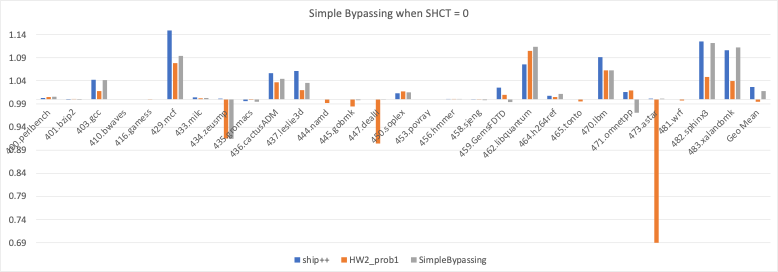
\includegraphics[width=0.9\textwidth]{figs/Picture4.png}
\caption{Simple bypassing when SHCT=0}
\label{fig.Picture4}
\end{figure*}
Bypassing cache replacement can perform well and provide performance improvements in certain situations. When the working set of an application is significantly larger than the cache size, bypassing can help reduce cache pollution by avoiding the storage of blocks that are unlikely to be reused in the near future.  In cases where access patterns are irregular or non-sequential, bypassing can prevent the eviction of frequently accessed cache blocks by avoiding the replacement of blocks with a low likelihood of being accessed again soon. Bypassing can alleviate cache thrashing situations, where cache blocks are continuously evicted and replaced due to the working set size exceeding the cache capacity. By identifying and bypassing blocks with a low reusability potential, cache thrashing can be mitigated, improving overall system performance. If the current cache replacement policy is not achieving a satisfactory cache hit rate, bypassing can help improve cache performance by selectively bypassing blocks that are deemed less likely to be accessed in the near future. In scenarios where data is accessed in a streaming or one-time manner (e.g., multimedia processing or large dataset scans), bypassing cache replacement can prevent the unnecessary eviction of other potentially reusable blocks, ultimately improving cache hit rate and overall performance\cite{Gao2010}. \par
Consequently, in the context of this project, the bypassing strategy is considered ineffective when the majority of reuse distances exceed the number of cache ways present in a set (16). Although the SHCT can determine which signature's reuse distance is below 16, it cannot pinpoint the signature exhibiting the minimum reuse distance when the distance exceeds 16, leading to constant misses. Furthermore, when a signature is marked for bypassing, it is less likely to be accessed in the immediate future, resulting in a prolonged bypassing period. Simultaneously, it is crucial to ensure that bypassed data does not remain within sample sets to avoid hindering future access to such data.\par
Assuming a scenario with only four ways and an access pattern such as A B C D E A F G H I A..., combined with the condition that a block is marked for bypassing after two misses, as observed with the "A" pattern in the example, despite "A" possessing the smallest reuse distance, it might still be bypassed and consequently never accessed in the future. It becomes evident that the performance would be unsatisfactory.\par
To address the issue of cache thrashing, an additional parameter is introduced to count valuable data, such as enumerating the instances of "less than 2" in the Re-Reference Production Value (RRPV). Upon the counter value exceeding a pre-established threshold, determined to be 14 after conducting numerous experiments, bypassing will be implemented. Furthermore, a verification process will be employed to determine if the data is within the sample set. If the data is present in the sample set, it will adhere to the SHIP++ policy; if not, bypassing will be executed.\par 
The results are illustrated in fig. \ref{fig.Picture5}. As demonstrated by this figure, the performance of our policy significantly surpasses that of SHIP++ for benchmarks such as 462. Additionally, improvements are observed for the previously underperforming 434 benchmark.\par 

\begin{figure*}[htbp]
\centering
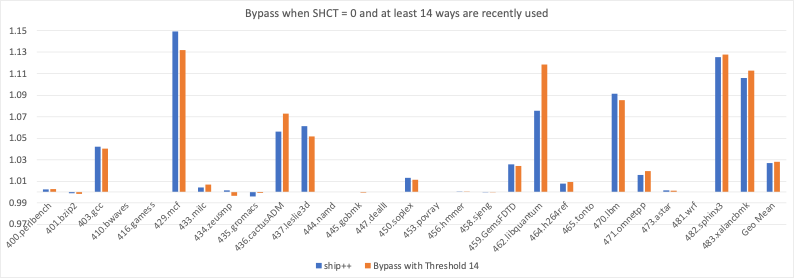
\includegraphics[width=0.9\textwidth]{figs/Picture5.png}
\caption{Bypassing when SHCT=0 and at least 14 ways are recently used}
\label{fig.Picture5}
\end{figure*}

\subsection{The utilization of SHCT}
When the initial value of the SHCT is set to 1, it is noted that the maximum value of the SHCT consistently stays at 1, even after 100 million accesses. This pattern is also persistently observed when the initial values are assigned as 2 and 5. Consequently, this suggests that a considerable portion of the SHCT table remains unutilized, leading to inefficiency and the squandering of resources.
\begin{figure}[htbp]
\centering
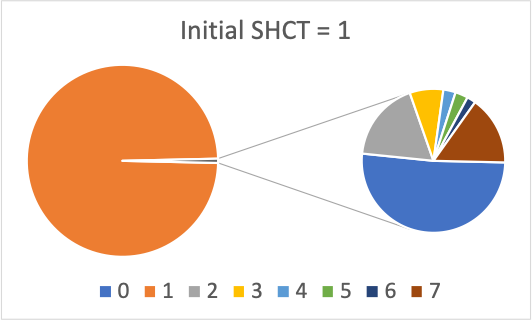
\includegraphics[width=0.4\textwidth]{figs/Picture1.png}
\caption{Initial SHCT = 1}
\label{fig.Picture1}
\end{figure}

\begin{figure}[htbp]
\centering
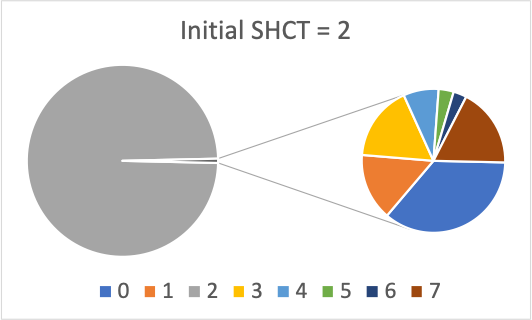
\includegraphics[width=0.4\textwidth]{figs/Picture2.png}
\caption{Initial SHCT = 2}
\label{fig.Picture2}
\end{figure}

\begin{figure}[htbp]
\centering
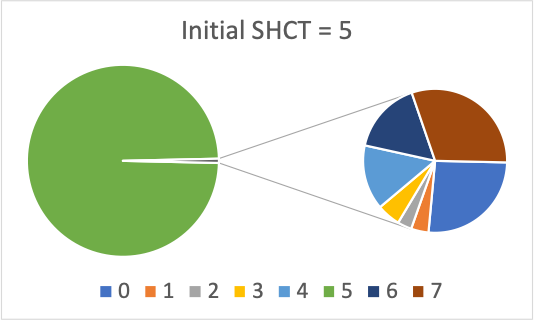
\includegraphics[width=0.4\textwidth]{figs/Picture3.png}
\caption{Initial SHCT = 5}
\label{fig.Picture3}
\end{figure}

SHCT has 16K entries, with each entry consisting of 3 bits. Subsequently, three minor experiments are conducted to further investigate the system.
\begin{itemize}
    \item \(Test 1\): try the smaller size entries like 4K entries,  and keep the same 3 bits.
    \item \(Test 2\): keep the same size entries, try the smaller number bits like 2 bits.
    \item \(Test 3\): try the smaller size entries like 4K entries, and also smaller number bits like 2 bits.
\end{itemize}
The result is illustrated in the fig. \ref{fig.Figure6}. From this depiction, it is evident that the geometric mean across the various configurations is quite similar. Consequently, it is possible to reduce the size of the SHCT table, thereby decreasing the hardware storage requirements.
\begin{figure*}[htbp]
\centering
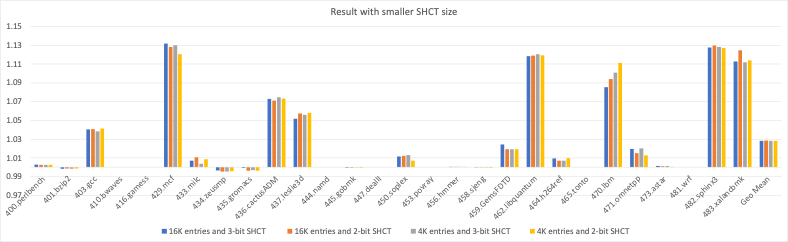
\includegraphics[width=0.9\textwidth]{figs/Picture6.png}
\caption{Result with smaller size}
\label{fig.Figure6}
\end{figure*}

% experiment

\section{Experiments}
\subsection{Experimental setup}
Our project will be divided into three parts: a 2-bit counter to track the re-reference Interval Prediction Value(RRPV); The Signature HIstory Counter Table(SHCT) of saturating counters to learn the re-reference behavior of a signature and bypassing topology.
\begin{itemize}
    \item \(RRPV\): 2-bit counter. As shown in fig. \ref{fig.RRPV}, upon a hit to the line, the RRPV is reset to 0. In the event of a miss, the victim is identified by commencing the search from way 0 and locating the first line in the set with an RRPV of 3. If no such line is found, the RRPV of all lines in the set is incremented, and the search is conducted once more. The RRIP can insert the line with either a high-priority position (RRPV=2) or a low-priority position (RRPV=3). The selection of the insertion position can be determined either statically for all references, as in the case of SRRIP, or dynamically at runtime, as with DRRIP. 
    
\begin{figure}[htbp]
\centering
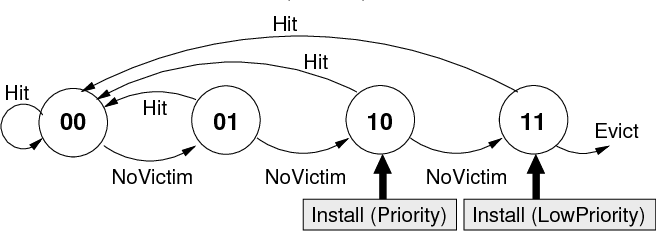
\includegraphics[width=0.5\textwidth]{figs/RRPV.png}
\caption{Re-reference Interval Prediction.}
\label{fig.RRPV}
\end{figure}

    \item \(SHCT\): 3-bit counter, as shown in fig. \ref{fig.SHCT}, SHIP necessitates the storage of two additional fields with each cache line: the signature (Program Counter, or PC, has been chosen for this project) and a single-bit to monitor the outcome of the cache insertion. The outcome bit, initially set to zero, is assigned a value of one only if the cache line is re-referenced. SHIP also employs a Signature History Counter Table (SHCT) of saturating counters, indexed by the signature associated with the cache line. Upon a hit to a cache line, SHIP increments the SHCT entry indexed by the signature stored with the cache line. Conversely, when a line is evicted from the cache without being re-referenced since insertion, SHIP decrements the SHCT entry indexed by the PC signature associated with the evicted cache line.
    
\begin{figure}[htbp]
\centering
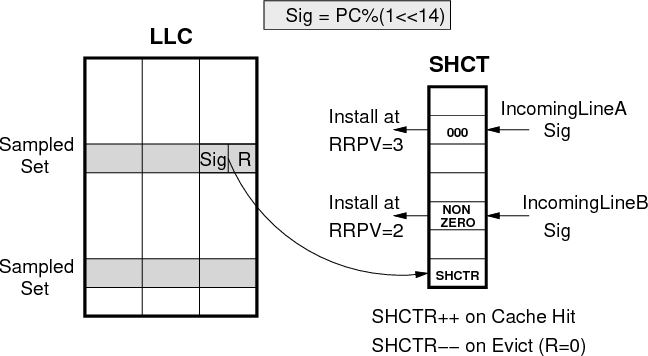
\includegraphics[width=0.5\textwidth]{figs/SHCT.png}
\caption{Signature History Counter Table.}
\label{fig.SHCT}
\end{figure}
    \item \(Bypassing\): The objective is to safeguard valuable data. Nevertheless, when the working set of data exceeds the cache size, resulting in a high rate of cache misses and the incessant eviction and loading of data, such as in the case of cache thrashing, bypassing becomes unfeasible. As a result, an approach is explored to quantify the number of valuable data elements in a specific manner and subsequently determine whether or not to execute bypassing.
\end{itemize}


\subsection{Discussion}
As demonstrated in Table. \ref{table.util}, the proposed policy outperforms SHIP++ in the current evaluation.
\begin{table}[htbp]
\caption{Result Summary}
\begin{center}
\begin{tabular}{|c|c|}
\hline
\textbf{Policy}&\textbf{GeoMean compared with LRU}\\
\hline
SHiP++(16K/3-bit SHCT) & 1.0268\\
\hline
Simple Bypass when SHCT = 0 & 1.0181\\
\hline
Bypass when SHCT = 0 \\and at least 14 recently used ways & 1.028\\
\hline
Same policy but 16k/2-bit SHCT &   1.0284\\
\hline
Same policy but 4k/3-bit SHCT  &   1.0282\\
\hline
Same policy but 4k/2-bit SHCT  &   1.0281\\
\hline
\end{tabular}
\label{table.util}
\end{center}
\end{table}
Also, there are many other ways to improve the utilization of the SHCT table.
\begin{itemize}
    \item \(Adaptive sizing\): Dynamically adjusting the size of the SHCT table based on the workload characteristics can help in maintaining an optimal table size, reducing hardware storage requirements without sacrificing performance.
    \item \(Intelligent initialization\): Instead of initializing all SHCT entries with the same value, consider using a smarter initialization strategy based on prior knowledge of the workload or by learning during an initial warm-up phase. This can help improve prediction accuracy and reduce the time it takes for the table to become useful.
    \item \(Aging mechanisms\): Implement an aging mechanism to periodically decrement or reset the counters in the SHCT table. This prevents counters from becoming saturated and allows the table to adapt to changes in access patterns over time.
    \item \(Multi-level SHCT\): Introduce a hierarchical SHCT structure with multiple levels to capture and predict different levels of re-reference intervals. This can provide more granular control over cache replacement decisions and improve prediction accuracy.
    \item \(Signature refinement\): Enhance the signature generation process to better differentiate between different data elements and their access patterns. This could include incorporating additional information, such as memory address bits or instruction-level information, to create more distinct and meaningful signatures.
    \item \(Hybrid approaches\): Combine SHCT with other cache replacement policies or prediction techniques to leverage the strengths of different approaches and improve overall cache performance.
\end{itemize}

% Conclusion

\section{Conclusion}
In conclusion, this discussion has primarily focused on cache replacement policies, including LRU, SHIP, and SHIP++, as well as the utilization of Signature History Counter Tables (SHCT) and bypassing techniques. The limitations of traditional LRU policy have led to the exploration of more advanced alternatives, such as SHIP and SHIP++, which incorporate adaptive mechanisms and data-driven techniques to improve cache performance.

The SHIP++ policy builds upon the original SHIP by using SHCT more effectively, thereby enhancing the prediction accuracy of re-reference intervals and making better-informed cache replacement decisions. The combination of improved signature generation, adaptive SHCT updates, and bypassing techniques allows SHIP++ to deliver enhanced performance compared to LRU and the original SHIP.

Furthermore, the implementation and analysis of various bypassing strategies and counter values have revealed the importance of optimizing cache performance and resource utilization. By carefully tuning the parameters and addressing the challenges of cache thrashing, significant improvements in cache performance have been achieved in various benchmarks.

As cache management continues to play a critical role in modern computer architecture, further research and exploration of advanced cache replacement policies, such as SHIP++, will contribute to the development of more efficient and high-performing memory systems.

\bibliographystyle{IEEEtran}
\bibliography{refs}
\end{document}
